\documentclass[parskip=full]{scrreprt}

\usepackage[english]{babel}
\usepackage[utf8]{inputenc}
\usepackage{csquotes}
\usepackage[backend=biber]{biblatex}
\addbibresource{mainreport.bib}

\usepackage{graphicx}
  \graphicspath{ {./graphics/} }
\usepackage{url}
\usepackage{varioref}
\usepackage{tabularx}
  \newcolumntype{L}{>{\raggedright\arraybackslash}X}
\usepackage[version=4]{mhchem}
  
\author{Arin Wongprommoon\\University of Cambridge}
\title{Optimising production of citramalate based on the \emph{E. coli} kinetic model}
\subtitle{Project Report}
\date{17 August 2018}

\begin{document}

\maketitle

\tableofcontents

\begin{abstract}
  Using living organisms to synthesise chemicals is an alternative to synthesising chemicals from fossil fuels, as it serves as a renewable resource with potentially high efficiency and low cost. The procedures can be sped up by optimising conditions using mathematical models. Citramalate ((2S)-2-Hydroxy-2-methylbutanedioate) is a chemical of industrial interest as it can be a precursor for methacrylic acid, a monomer for the production of plastics. 
  
  The project aimed to find conditions to maximise the production of citramalate using modelling approaches. In this project, an existing kinetic model for \emph{E. coli} metabolism was extended by adding a reaction that produces citramalate from acetyl coenzyme A and pyruvate. \emph{E. coli} was chosen as the model organism as its metabolism is very well characterised in the literature. The project employed Python and libraries specific to genetic algorithms, modelling, and manipulating information presented in SBML (systems biology markup language).
  
  First, the effect of $V_{max}$ values of enzymes in the kinetic model~\cite{millard_metabolic_2017} on productivity of citramalate was investigated. $V_{max}$ values were chosen as a parameter as it can be easily tested \emph{in vivo} by relying on the principle that $V_{max}$ is proportional to enzyme concentration. The differential evolution genetic algorthim was then employed to compute the set of $V_{max}$ values of enzymes that optimises the production of citramalate, assuming Michaelis-Menten kinetics.
  
  In the second part of the project, information from the kinetic model was used to enrich the stoichiometric model~\cite{orth_comprehensive_2011}. More specifically, information about the possible values of fluxes through each reaciton was used to set the boundaries for each reaction in a stoichiometric model. Flux balance analysis (FBA) was then performed to evaluate the highest possible flux through the citramalate-producing reaction as a proxy for citramalate productivity. The composition of the Lund medium~\cite{eastham_process_2015} was studied in an attempt to create boundaries for relevant uptake reactions.
  
  The project took place at the Cambridge Systems Biology Centre, Department of Biochemistry, in Prof Steve Oliver's group. Research associate Dr Jorge J\'ulvez supervised me throughout the project. The project was entirely computational, and ran from 25 June 2018 to 17 August 2018.
\end{abstract}

\chapter*{Introduction}
\label{ch:intro}

The project concerns two models of \emph{E. coli} metabolism: a kinetic model described by Millard \emph{et al} in 2017~\cite{millard_metabolic_2017} and a stoichiometric model described by Orth \emph{et al} in 2011~\cite{orth_comprehensive_2011}. The kinetic model concerns a smaller set of reactions than the stoichiometric model, but it contains information about initial conditions (substrate concentrations and flux through reactions) which the stoichiometric model lacks.

The kinetic model contains 68 reactions, 49 of which include $V_{max}$ as a parameter. Of these, 41\footnote{ACEA, ACEB, ACK, ACN\_1, ACN\_2, ACS, ATP\_syn, CITRA\_SYN, CYTBO, EDA, EDD, ENO, FBA, FBP, FUMA, GDH, GLT, GND, GPM, LPD, MAD, MDH, MQO, PCK, PDH, PFK, PGI, PGK, PGL, PIT, PPC, PPS, PTA, PYK, RPE, RPI, SDH, SK, SQR, TPI, and ZWF} correspond to real enzyme-catalyzed reactions in \emph{E. coli}. To investigate citramalate production, a 69th reaction, modelling the reaction:

\begin{center}
  acetyl-CoA + pyruvate + \ce{H2O} $\rightarrow$ CoA-SH + \ce{H^+} + citramalate
\end{center}

with the kinetic law

\[
  \frac{\mathrm{d}[citramalate]}{\mathrm{d}t} = 
  \frac{V_{max} \cdot [acetyl-CoA]}{[acetyl-CoA] + K_{m}}
\]

assuming pyruvate is saturating. The $V_{max}$ is set to 4 mM s\textsuperscript{-1} and $K_{m}$ to 0.495 mM in the modified model.

Citramalate productivity is defined as $\mu Y_{P/S}$, where $\mu$ is the growth rate in reciprocal time units (h\textsuperscript{-1} in this project) and $Y_{P/S}$ is defined as mass of product over mass of substrate, which is glucose in this context. Manipulating the SBML file required the Python library \texttt{libsbml} and running simulations employed the \texttt{roadrunner} module. Throughout the project, the simulations were from 0 to 7200 seconds, at which steady-state is attained for almost all the conditions (also see section~\vref{sec:couples}) %change this to a subsection investigating steady-state later

The stoichiometric model contains 2,584 reactions, and I have mapped 57 of them to their equivalents in the kinetic model (more details in section~\vref{sec:mapping}). By default, most of these reactions are unbounded (Orth \emph{et al}~\cite{orth_comprehensive_2011} provided details about this). In a similar vein to the kinetic model, a 2,585th reaction for citramalate production was added to the stoichiometric model using the COBRA module in Python. However, no kinetic parameters were added, as stoichiometric models do not contain this information. In addition to the citramalate synthesis reaction, a sink reaction to allow citramalate to leave the system was also added.

\chapter{Investigating the kinetic model}
\label{ch:kinetic}

%(Maybe write the purpose of doing this here? But I think the abstract and the introduction suffice)

\section{Varying $V_{max}$ values of one reaction at a time}
\label{sec:onereac}

Here I investigated the relationship between the value of $V_{max}$ of each reaction in the kinetic model and the resulting citramalate productivity at steady state -- i.e.\ after two hours. I varied the $V_{max}$ values of each of the 49 reactions\footnote{ACEA, ACEB, ACK, ACN\_1, ACN\_2, ACS, ATP\_MAINTENANCE, ATP\_syn, CITRA\_SYN, CYTBO, EDA, EDD, ENO, FBA, FBP, FUMA, GDH, GLT, GND, GPM, GROWTH, LPD, MAD, MDH, MQO, NADH\_req, NDHII, PCK, PDH, PFK, PGI, PGK, PGL, PIT, PPC, PPS, PTA, PYK, RPE, RPI, SDH, SK, SQR, TPI, XCH\_ACE1, XCH\_ACE2, XCH\_GLC, XCH\_ZWF} in the kinetic model that include $V_{max}$ as a parameter. The ranges 0.1--1.0 $V_{max}$ and 0.1--10.0 $V_{max}$, where $V_{max}$ is the wild-type $V_{max}$ for that particular reaction as specified in the SBML file. I used 100 data points for each plot. Figure~\ref{fig:onereacsample} is an example of such a plot.

\begin{figure}[htbp]
  \centering
  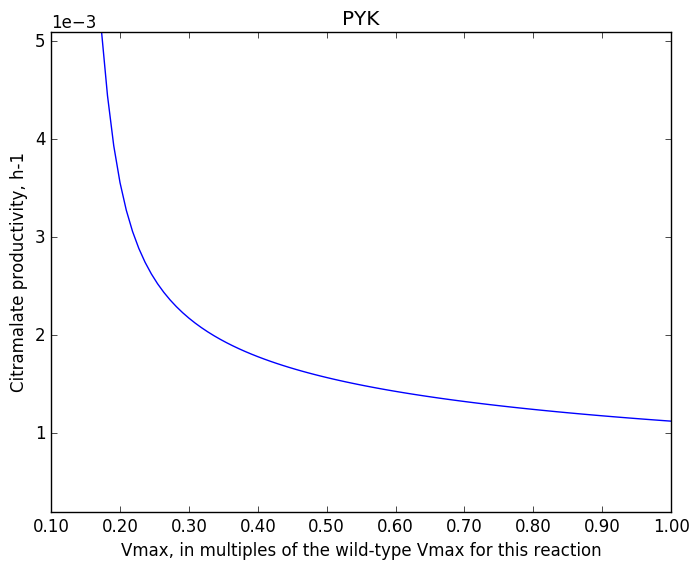
\includegraphics[scale=0.5]{onereacsample}
  \caption{Example of a one-reaction plot: the reaction PYK}
  \label{fig:onereacsample}
\end{figure}

For some enzymes, varying $V_{max}$ values have a greater effect on citramalate productivity than others. I quantified this effect based on the data points of the 0.5 -- 2.0 $V_{max}$ plots\footnote{created early in the project, not included in the final results. I only mention them here because I used information from them in later parts of the project} as follows:

\[
effect = \frac{(max - min)}{(0.5 \cdot (max + min)}
\]

This is the difference between the maximum and minimum productivities obtained over the range, relative to the average, which represents where the value of productivity is. I intended to find the extent of variation from the `typical' value of productivity around this range. Granted, this isn’t the best way to analyse. I’ve tried regression, but it didn’t seem very informative.

This identified CITRA\_SYN, GLT, LPD, GROWTH, ATP\_MAINTENANCE, GDH, ATP\_SYN, ACEA, PYK, and ZWF as among the enzymes that had the greatest effects. Millard et al (2017) listed CYTBO, ZWF, GDH, GLT, and GROWTH as the enzymes found to have the largest shares of flux control (and also exert the strongest controls on concentration). And looking at figure 2A and figure 2B, they are followed by the likes of LPD, ATP\_MAINTENANCE, ACEA, ATP\_SYN, and PYK

XCH\_XXX for ACE, GLC, and P have no bearing on productivity. Surprisingly, ACS (acetyl CoA synthetase), ACK (acetate kinase), and PTA (phosphate acetyltransferase), which are all directly related to controlling acetyl CoA levels, do not seem to have a significant bearing on productivity.

Enzymes found to have the largest shares of flux control unsurprisingly create the plots that demonstrate the greatest change in citramalate productivity in response to Vmax changes. So what's more interesting are:\\
CYTBO -- has a less effect on productivity as would be expected by this explanation.\\
PYK. It doesn't exert a lot of control over fluxes. However, the citramalate reaction uses up pyruvate, so that might explain the difference. PYK is also a control point of glycolysis.

These enzymes have inflection points in their plots (which is surprising, but Prof Oliver said it’s likely due to the feedback control mechanisms). I’ve calculated some of these (absolute values)
CYTBO: 4.9325456122 to 5.0894110204\\
PFK: 0.1410191204 to 0.1444217265\\
GDH: 4.3682353265 to 4.5274017959\\
EDA: 0.0134480582 to 0.0148719702\\
MQO: 1.4811924694 to 1.5661015918\\
CITRA\_SYN: 0.4734693878 to 0.5469387755

\section{Varying $V_{max}$ values of two reactions at a time}
\label{sec:couples}

Aliquam erat volutpat. Nam sed felis dui. Suspendisse rhoncus dui vel mi accumsan, malesuada tempus ligula aliquet. Nulla purus dui, feugiat non justo tempor, consectetur vehicula sem. Aenean at libero ipsum. Suspendisse aliquet nec metus sed tincidunt. Donec vel sapien id diam condimentum cursus.

\section{Using differential evolution}
\label{sec:de}

Orci varius natoque penatibus et magnis dis parturient montes, nascetur ridiculus mus. Suspendisse pellentesque quis nunc eget feugiat. Praesent eu neque dapibus, tincidunt dolor eu, elementum neque. Donec sit amet augue justo. Suspendisse condimentum lectus sed tellus mollis, non commodo ipsum porttitor. Nam efficitur, leo id egestas feugiat, augue odio hendrerit ligula, non tempor mi elit a quam. Sed sagittis pulvinar lorem, non ornare metus tempor nec. Nullam interdum rutrum nulla non suscipit. Ut orci enim, molestie in rhoncus ut, placerat in nunc. Nulla scelerisque ullamcorper nibh, quis commodo augue laoreet faucibus. Donec fermentum faucibus venenatis. In convallis, ligula ut accumsan gravida, lectus quam gravida metus, nec tempor ipsum mi eu nulla. Nulla aliquam vestibulum felis, interdum tincidunt velit ultrices ac. Curabitur a libero sagittis, pulvinar urna vel, auctor urna. Donec tempus sem mi, sit amet ornare mi suscipit vitae.

\chapter{Enriching the stoichiometric model}
\label{ch:stoich}

Donec porta ipsum fermentum arcu semper lacinia. Mauris sodales non sapien non auctor. Pellentesque nec odio vitae felis varius sodales. Proin eu velit ac nunc congue mollis. Nullam ut lectus nec ligula fermentum finibus. Fusce maximus aliquet nisi, rhoncus scelerisque felis sollicitudin vulputate. Maecenas molestie enim at lacus pharetra, eget interdum leo imperdiet. Nunc ut placerat velit. Cras volutpat a lorem sit amet euismod. Nullam pretium suscipit nibh vel placerat. Curabitur maximus, tellus ut tempor blandit, tellus elit suscipit lectus, vitae rhoncus mi purus condimentum mi. Vivamus congue lacus libero, ac rhoncus leo convallis sit amet. Integer vel accumsan lorem. Sed vitae lacus quis nisl consequat tincidunt. Nunc ut urna quam. 

\section{Mapping reactions in the kinetic model to the stoichiometric model}
\label{sec:mapping}

In hac habitasse platea dictumst. Sed a metus ante. Pellentesque eget imperdiet nulla. Sed convallis sagittis augue at vehicula. Nulla nec efficitur arcu. Suspendisse hendrerit massa nec mauris fermentum, eu iaculis tortor vehicula. Vestibulum sed tristique nulla.

Integer vel ullamcorper augue, nec congue quam. Quisque luctus molestie lectus quis sagittis. Vivamus facilisis placerat eros ut aliquet. Aliquam volutpat elit eget risus gravida, sed luctus erat interdum. In id suscipit tellus, a mollis elit. Sed pulvinar, diam et aliquam varius, lectus risus rutrum libero, vitae posuere urna odio eget neque. Etiam aliquet ante quis porttitor lobortis. Nullam elit sapien, pharetra at libero non, ullamcorper efficitur ex. Etiam laoreet ullamcorper orci, vitae pretium risus convallis et. Proin et orci felis. In hendrerit lectus eget nisl tincidunt, ut faucibus justo tempus. Nulla at elit auctor, aliquet orci et, euismod magna.

\section{Creating boundaries for FBA}
\label{sec:bounds}

Vestibulum placerat purus vel nisl imperdiet, eu condimentum ex semper. Sed semper dignissim enim quis condimentum. Suspendisse potenti. Vivamus molestie tortor vitae volutpat ultrices. Aenean nec accumsan sapien. Suspendisse potenti. Donec dignissim felis sed ex accumsan venenatis. Suspendisse varius mi sed mattis sagittis. Donec dapibus rhoncus ipsum, non mattis ex finibus sed. Quisque eget volutpat justo.

Etiam massa tellus, tincidunt ut metus at, volutpat viverra lectus. In sapien velit, tempor vitae vestibulum eu, lobortis dictum turpis. Aliquam blandit finibus venenatis. Quisque vestibulum viverra tellus, non bibendum ex molestie in. Maecenas non ante odio. Donec iaculis at nunc sed luctus. Suspendisse iaculis nibh eget eleifend tempus. Vestibulum porta ultrices volutpat. Donec semper lorem vitae hendrerit ultricies.

\section{Flux balance analysis}
\label{sec:fba}

Nullam lorem ligula, lacinia sit amet condimentum eu, aliquet vel lorem. Nam ut mollis nisl. Vestibulum ante ipsum primis in faucibus orci luctus et ultrices posuere cubilia Curae; Aliquam blandit, eros ac elementum consectetur, sem ante suscipit ante, vitae laoreet lectus elit ac sem. Fusce nunc velit, ullamcorper quis magna semper, tempus sodales magna. Nullam vel pharetra libero. Nam rutrum posuere neque quis suscipit. Donec tristique sapien orci. Ut eros orci, malesuada id leo nec, bibendum semper metus. Pellentesque ut dictum lectus. Donec auctor dapibus arcu et tincidunt. Sed cursus est posuere felis lacinia, quis sollicitudin erat vestibulum. Proin lobortis felis eget neque suscipit mattis.

Phasellus leo augue, porta et consequat gravida, ullamcorper eu ligula. Curabitur eu neque vitae enim porta egestas. Sed commodo ligula ex, at faucibus augue convallis eu. Suspendisse tortor augue, lacinia sit amet nisi vel, posuere varius turpis. Quisque ut mauris eget arcu luctus blandit. Vestibulum egestas vehicula diam non accumsan. Suspendisse pulvinar nec tellus vitae luctus.

\section{Using information from the Lund medium}
\label{sec:lund}

Pellentesque imperdiet quam vitae commodo pellentesque. Donec vitae eros dolor. Phasellus sit amet euismod augue. Integer dictum a arcu vitae ornare. Quisque interdum nibh eu arcu gravida dapibus sit amet et tortor. Nam laoreet ultrices dapibus. Cras tincidunt sem sodales massa rutrum efficitur a non arcu. Etiam porta massa a fermentum maximus. Curabitur sit amet pulvinar justo, sed congue magna. Nulla non sem non augue rhoncus rutrum ut in risus. Aliquam varius, ipsum vitae laoreet dignissim, odio augue convallis dolor, quis mollis mauris sem eget nibh. Nunc finibus turpis ac lectus volutpat, eu egestas ex porta. Cras ante justo, blandit sit amet viverra non, rhoncus sodales mi. Vestibulum ante ipsum primis in faucibus orci luctus et ultrices posuere cubilia Curae;

\chapter{Remarks}
\label{ch:remarks}

Donec at rutrum tellus, ut posuere urna. Nulla facilisi. Quisque ut orci tincidunt, ultricies eros sed, ultrices purus. Praesent scelerisque nunc urna, in pharetra augue pharetra ut. In quis quam consectetur, finibus orci sit amet, molestie massa. Nullam vel dictum lorem. 

\section{Issues in the project}
\label{sec:issues}

Memory leak, things that don't make sense, etc. Things that get in the way of me making revolutionary discoveries.

Vestibulum sed est molestie, feugiat justo vitae, aliquam augue. Ut accumsan massa dignissim, maximus nulla at, imperdiet ligula. Donec vitae tortor vitae libero dapibus maximus. Fusce a enim faucibus, sollicitudin sapien nec, maximus nibh. Morbi pharetra egestas lorem, non semper arcu faucibus vitae. Morbi vehicula urna ac odio blandit gravida. Integer id magna pharetra, gravida odio et, pulvinar magna. Praesent consequat elementum mollis.

\section{Future direction and suggestions}
\label{sec:future}

Nunc orci justo, ultricies id pharetra a, consequat at dolor. Curabitur posuere nisl eget leo viverra, non cursus nunc consectetur. Fusce non turpis non sem porttitor cursus id a lacus. Mauris iaculis sit amet risus ut viverra. Nunc eget arcu magna. Donec quis suscipit metus. Donec aliquet imperdiet consectetur. Ut tempus, dui et sodales posuere, diam est sagittis est, nec consectetur mi dolor nec mi. Ut in lacus vitae sapien lacinia aliquam in tincidunt nisi. Etiam non pretium justo. Phasellus augue lectus, condimentum vel orci et, suscipit semper dolor. Fusce at finibus nulla.

\section{Notes about files}
\label{sec:files}

Notes about the scripts, text files, image files, spreadsheets etc.\ used. Notes about Git/GitHub.

Sed nec erat iaculis lectus rhoncus ornare. Duis ante ex, sodales sed mi sed, blandit venenatis dui. Donec vel ornare odio, laoreet viverra felis. Phasellus aliquam mi et sollicitudin fermentum. Ut vitae mollis lacus. Sed tempor nulla at rutrum iaculis. Vestibulum convallis elementum nibh, fermentum porttitor leo vulputate eget. Sed vel sagittis elit, eu faucibus ante. Aliquam erat volutpat. Donec mattis sit amet ante quis luctus. Fusce lectus risus, molestie at tincidunt non, consectetur nec massa. Duis arcu justo, lacinia ut nulla tristique, congue interdum purus. Maecenas finibus, urna eu mollis commodo, nisi metus tincidunt velit, at convallis libero justo id turpis. Etiam iaculis sodales quam vitae fringilla. 

\chapter*{Appendix}
\label{ch:appendix}

%\section

% Here I intend to put lists or figures that would be annoying if in the main text

\nocite{*}
\printbibliography

\end{document}
